\documentclass{article}
\usepackage{amsthm, amssymb, amsmath,verbatim}
\usepackage[margin=1in]{geometry}
\usepackage{enumerate}
\usepackage{enumitem}
\usepackage{graphicx}



\newtheorem*{claim}{Claim}
\newtheorem{ques}{Question}


\title{CSE 150 Homework 1}
\date{Fall 2018}
\author{Pedro Sousa Meireles}
\begin{document}

\maketitle
\section{Probabilistic reasoning}

\flushleft M = children have meltdown

L = I'll be late
\bigbreak
Data given by the question:

$P(M=1) = 0.01$

$P(L=1|M=1) = 0.98$

$P(L=1|M=0) = 0.03$
\bigbreak

Also:

\begin{align*}
P(L=1) &=P(L=1|M=1) \cdot P(M=1)+P(L=1|M=0) \cdot P(M=0)\\
&=0.98 \cdot 0.01 + 0.03 \cdot (1-0.01)\\
&=0.0297
\end{align*}
\bigbreak

The question says that I am late to campus (L = 1). Then what is requested is $P(M=1|L=1)$.

Using Bayes rule whe have $P(M=1|L=1)=\frac{P(L=1|M=1)*P(M=1)}{P(L=1)}$

\begin{align*}
P(M=1|L=1) & = \frac{0.98*0.01}{0.0297}\\
& = 0.3398
\end{align*}

\section{Conditioning on background evidence}

\begin{enumerate}[label=(\alph*)]
\item 
Product Rule: $$P(X, Y|E)=P(X|Y,E) \cdot P(Y|E)$$
By isolating the term $P(X|Y,E)$ we get:
$$P(X|Y,E)=\frac{P(X, Y|E)}{P(Y|E)}$$
Then, applying the Product rule again to $P(X, Y|E)$ we have:
$$P(X|Y,E)=\frac{P(Y|X,E) \cdot P(X|E)}{P(Y|E)}$$

\item
Applying the definition of conditional probability to $P(X|E)$ we have:
$$P(X|E)=\frac{P(X,E)}{P(E)}$$
Now applying the marginalization over Y in the numerator:
$$P(X|E)=\frac{\sum_{j} P(X,E, Y=y_j)}{P(E)}=\sum_{j}\frac{P(X,E, Y=y_j)}{P(E)}$$
Applying the definition of conditional probability again to each term of the sum we have:
$$P(X|E)=\sum_{j}P(X, Y=y_j|E)$$
\end{enumerate}

\section{Conditional independence}

\begin{enumerate}[label=(\roman*)]
\item
\underline{Proof that (ii) is true:} \bigbreak
Using the product rule for conditional probabilities in $P(X,Y|E)$ we have:
$$P(X,Y|E)=P(X|Y,E) \cdot P(Y|E)$$
Isolating $P(X|Y,E)$ we have:
$$P(X|Y,E) = \frac{P(X,Y|E)}{P(Y|E)}$$
Now using the statement (i):
$$P(X|Y,E) = \frac{P(X|E) \cdot P(Y|E)}{P(Y|E)}=P(X|E)$$

\underline{Proof that (iii) is true:}\bigbreak
Using the product rule for conditional probabilities in $P(X,Y|E)$ we have:
$$P(X,Y|E)=P(Y|X,E) \cdot P(X|E)$$
Isolating $P(Y|X,E)$ we have:
$$P(Y|X,E) = \frac{P(X,Y|E)}{P(X|E)}$$
Now using the statement (i):
$$P(Y|X,E) = \frac{P(X|E) \cdot P(Y|E)}{P(X|E)}=P(Y|E)$$

\item
\underline{Proof that (i) is true:} \bigbreak
Using the product rule for conditional probabilities in $P(X,Y|E)$ we have:
$$P(X,Y|E)=P(X|Y,E) \cdot P(Y|E)$$
Now using the statement (ii) in $P(X|Y,E)$:
$$P(X,Y|E) = P(X|E) \cdot P(Y|E)$$

\underline{Proof that (iii) is true:}\bigbreak
Using Bayes' rule for conditional probabilities we have:
$$P(Y|X,E)=\frac{P(X|Y,E) \cdot P(Y|E)}{P(X|E)} $$
Now using the statement (ii) in $P(X|Y,E)$:
$$P(Y|X,E) = \frac{P(X|E) \cdot P(Y|E)}{P(X|E)}=P(Y|E)$$

\item
\underline{Proof that (i) is true:} \bigbreak
Using the product rule for conditional probabilities in $P(X,Y|E)$ we have:
$$P(X,Y|E)=P(Y|X,E) \cdot P(X|E)$$
Now using the statement (ii) in $P(Y|X,E)$:
$$P(X,Y|E) = P(Y|E) \cdot P(X|E)$$

\underline{Proof that (ii) is true:}\bigbreak
Using Bayes' rule for conditional probabilities we have:
$$P(X|Y,E)=\frac{P(Y|X,E) \cdot P(X|E)}{P(Y|E)} $$
Now using the statement (ii) in $P(Y|X,E)$:
$$P(X|Y,E) = \frac{P(Y|E) \cdot P(X|E)}{P(Y|E)}=P(X|E)$$
\end{enumerate}

\section{Creative writing}

\begin{enumerate}[label=(\alph*)]
\item
X = Having skin cancer

Y = Using sunscreen

Z = Going often to the beach

$P(X=1|Z=1)>P(X=1)$: The probability of having skin cancer is bigger if you go often to the beach.

$P(X=1|Y=1,Z=1)<P(X=1|Z=1)$: If you go often to the beach, the probability of having skin cancer is smaller if you use sunscreen.

\item
X = Get an A

Y = Do all homeworks

Z = Study frequently

$P(X=1) < P(X=1|Y=1) < P(X=1|Z=1,Y=1)$: The probability to get an A increases if you do all homework and grows even bigger if you also study often.

\item 
X = Team A wins

Y = Team B wins

Z = Team A and Team B are not playing agains each other

$P(X,Y|Z = P(X|Z) \cdot P(Y|Z))$: The results of Team A's and Team B's games are independent because they are not playing against each other.

$P(X=1,Y=1)<P(X=1)P(Y=1)$: The probability that both teams win is lower than the product of their probabilities of winning, because they may been playing against each other.
\end{enumerate}

\section{Probabilistic inference}

Given data:

$P(B=1)=0.001$

$P(E=1)=0.005$

$P(J=1|A=0)=0.1$

$P(J=1|A=1)=0.93$

$P(M=1|A=0)=0.01$

$P(M=1|A=1)=0.65$

$P(A=1|E=0,B=0)=0.002$

$P(A=1|E=0,B=1)=0.96$

$P(A=1|E=1,B=0)=0.35$

$P(A=1|E=1,B=1)=0.98$
\bigbreak
Trivial data:

$P(B=0)=0.999$

$P(E=0)=0.995$
\bigbreak
Data calculated in lecture:

$P(B=1|A=1)=0.2044$

$P(A=1)=0.00469636$

$P(A=0)=0.99530364$

$P(A=1|E=1)=0.35063$

$P(A=0|E=1)=0.64937$

\bigbreak
\begin{enumerate}[label=(\alph*)]
\item
Probability calculated in lecture.
$$P(B=1|A=1)=0.2044$$

\item
$P(B=1|A=1,E=0) = \frac{P(A=1|B=1,E=0) \cdot P(B=1|E=0)}{P(A=1|E=0)}$  (Bayes rule)

We already know $P(A=1|B=1,E=0)=0.96$ and $P(B=1|E=0)=P(B=1)=0.001$ because B and E are conditionally independent.
Now we must find out the value of $P(A=1|E=0)$:

\begin{align*}
P(A=1|E=0) & = \sum_{b}P(A=1,B=b|E=0) && \text{(Marginalization over B)}\\
& = \sum_{b}P(A=1|B=b,E=0) \cdot P(B=b|E=1) &&  \text{(Product rule)}\\
& = \sum_{b}P(A=1|B=b,E=0) \cdot P(B=b) && \text{($P(B|E)=P(B)$)}\\
& = 0.002 \cdot 0.999 + 0.96 \cdot 0.001\\
& = 0.002958\\
\end{align*}

Replacing values:

$$P(B=1|A=1,E=0) = \frac{0.98 \cdot 0.001}{0.002958} = 0.3313$$

\item
Probability calculated in lecture.
$$P(A=1|J=1)=0.0420375$$

\item
$P(A=1|J=1,M=1) = \frac{P(J=1,M=1|A=1) \cdot P(A=1)}{P(J=1,M=1)}$  (Bayes rule on $Y=(J=1,M=1)$)

We already know $P(A=1)$, so we have to discover $P(J=1,M=1|A=1)$ and $P(J=1,M=1)$:

\begin{align*}
P(J=1,M=1|A=1) & =P(J=1|A=1,M=1) \cdot P(M=1|A=1) && \text{(Product rule)}\\
& =P(J=1|A=1) \cdot P(M=1|A=1) && \text{($P(J|A,M)=P(J|A)$)}
& = 0.93 \cdot 0.65\\
& = 0.6045
\end{align*}

\begin{align*}
P(J=1,M=1) & =\sum_{a}P(J=1,M=1,A=a) && \text{(Marginalization over A)}\\
& = \sum_{a}P(J=1|M=1,A=a) \cdot P(M=1|A=a) \cdot P(A=a) && \text{(Product rule)}\\
& = \sum_{a}P(J=1|A=a) \cdot P(M=1|A=a) \cdot P(A=a) && \text{($P(J|A,M)=P(J|A)$)}\\
& = 0.1 \cdot 0.01 \cdot 0.99530364 + 0.93 \cdot 0.65 \cdot 0.00469636\\
& = 0.00383425326
\end{align*}

Now, replacing the calculated values in the original formula:

$$P(A=1|J=1,M=1) = \frac{0.6045 \cdot 0.00469636}{0.00383425326} = 0.7404 $$

\item
$P(A=1|M=0)=P(M=0|A=1) \cdot P(M=0)$ (Product Rule)

We already know $P(M=0|A=1) = 1 - P(M=1|A=1) = 0.35$, so $P(M=0)$ remains to be found:

\begin{align*}
P(M=0) & =1-P(M=1)\\
& =1-\sum_{a}P(M=1,A=a) && \text{(Marginalization over A)}\\
& =1-\sum_{a}P(M=1|A=a) \cdot P(A=a) && \text{(Product rule)}\\
& = 1-(0.01 \cdot 0.00469636 + 0.65 \cdot 0.99530364)\\
& = 0.3530056704
\end{align*}

Replacing:

$$P(A=1|M=0)=0.35 \cdot 0.3530056704 = 0.1236$$

\item
$P(A=1|M=0,E=1)=\frac{P(M=0|A=1,E=1) \cdot P(A=1|E=1)}{P(M=0|E=1)}$ (Bayes rule)

We already know $P(M=0|A=1,E=1)=P(M=0|A=1)=1-P(M=1|A=1)=0.35$ (M and E are conditionally independent given A).
We also know $P(A=1|E=1)=0.35063$. Now, we have to find out the value of $P(M=0|E=1)$:

\begin{align*}
P(M=0|E=1) & =1-P(M=1|E=1)\\
& =1-\sum_{a}P(M=1,A=a|E=1) && \text{(Marginalization over A)}\\
& =1-\sum_{a}P(M=1|A=a,E=1) \cdot P(A=a|E=1) && \text{(Product rule)}\\
& =1-\sum_{a}P(M=1|A=a) \cdot P(A=a|E=1) && \text{($P(M|A,E)=P(M|A$)}\\
& = 1-(0.01 \cdot 0.64937 + 0.65 \cdot 0.35063)\\
& = 0.7655968
\end{align*}

Now, replacing in the original formula:

$$P(A=1|M=0,E=1)=\frac{0.35 \cdot 0.35063}{0.7655968}=0.1603$$
\end{enumerate}

\textbf{Analysis}

Comparing itens (a) and (b), the results follow commonsense patterns of reasoning, because the probability of burglary when the alarm sounds and there is no earthquake is bigger than the probability of burglary given that the alarm is on. In item (a), it is possible that another factor made the alarm sound, such as an earthquake, which is discarted in letter (b).\bigbreak

Comparing itens (c) and (d), the results also follow commonsense patterns of reasoning, because the probability of the alarm going off is bigger when more people call you.\bigbreak

Comparing itens (e) and (f), the results follow commonsense patterns of reasoning, because the probability of the alarm going off knowing that Maya didn't call is bigger when an earthquake happened.\bigbreak

\section{Kullback-Leibler distance}

\begin{figure}[h!]
  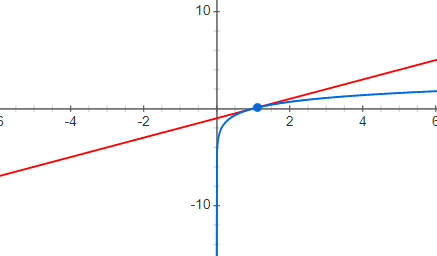
\includegraphics[scale=1]{graphic1.png}
  \centering
  \caption{Red: z-1, Blue: log(z)}
\end{figure}

\begin{enumerate}[label=(\alph*)]
\item
$\frac{\partial}{\partial z}(log(z)-(z-1))=\frac{1}{z}-1$

In $z=1$ the derivative is 0, which denotes it is a critic point. For $z>1$ the derivative is always negative, as $\frac{1}{z}-1<0$ for every z in range. 
For $0<z<1$ the derivative is always positive, as $\frac{1}{z}-1>0$ for every z in range. Thus, z=1 is the only critic point and is a global maximum. replacing z in the original inequality we have $log(1)\leq1-1$ which is true, for $0\leq0$. As it is proved this is the global maximum of the difference between both sides, the inequality is true with equality if and only if $z=1$;

\item
Defining $z_i=\frac{q_i}{pi}$ we can write:


\begin{align*}
KL(p,q) &=-\sum_i p_i \cdot log(z_i)\\
\intertext{We can use the relation proved on item (a) multiplied by -1} 
& =-\sum_i p_i \cdot log(z_i) >=  -\sum_ip_i \cdot (z_i-1)\\
& \geq -\sum_i p_i \cdot (\frac{q_i}{p_i}-1) & \text{($z_i=\frac{q_i}{pi}$)}\\
& \geq \sum_i (p_i-q_i)\\
& \geq \sum_i p_i- \sum_i q_i\\
& \geq 1-1 & \text{($\sum_i p_i=1$ and $\sum_i q_i=1$)}\\
& \geq 0
\end{align*}

As the result is due directly from the property proved on item (a), the equality of this inequality happens when $z=1$, which means $q_i=p_i$.

\item
$p_0=P(X=0|E)=0.25$

$p_1=P(X=1|E)=0.75$

$q_0=P(X=0|E')=0.66$

$q_1=P(X=1|E')=0.34$

$KL(p,q)=0.25 \cdot log(\frac{0.25}{0.66})+0.75 \cdot log(\frac{0.75}{0.34}) = 0.350650962$

$KL(q,p)=0.66 \cdot log(\frac{0.66}{0.25})+0.34 \cdot log(\frac{0.34}{0.75}) = 0.371730705$

$$KL(p,q) \neq KL(q,p)$$
\end{enumerate}

\end{document} 